\RequirePackage{fix-cm}
\documentclass[smallextended]{svjour3}
\smartqed
%Para funcionar o CITEP:
\usepackage[square,sort]{natbib}
%Para rodar em português com cedilha e hifenização certa.
\usepackage{graphicx,url}
\usepackage[brazil]{babel}   
\usepackage[utf8]{inputenc}  
\usepackage[toc,page]{appendix}
\journalname{Data Min Knowl Disc}
%
\begin{document}
\title{Detecção de Fraudes: Uma Revisão Sistemática
}
\subtitle{}
\titlerunning{Detecção de Fraudes: Uma Revisão Sistemática}
\author{Jean Avila Rangel         \and
	Maria Claudia Figueiredo Pereira Emer \and
	Adolfo Gustavo Serra Seca Neto
}
\institute{Jean Avila Rangel
\at Federal University of Technology - Paraná, 3165 Sete de Setembro Avenue, Curitiba, PR 80230-901, BRA
\and
Maria Claudia Figueiredo Pereira Emer \and Adolfo Gustavo Serra Seca Neto
\at Academic Department of Informatics, Federal University of Technology - Paraná, 3165 Sete de Setembro Avenue, Curitiba, PR 80230-901, BRA
\\\email{mciemer@gmail.com} 
\\
\and
Adolfo Gustavo Serra Seca Neto \\\email{adolfo@dainf.ct.utfpr.edu.br}
}
	\date{Received: date / Accepted: date}
	% The correct dates will be entered by the editor
	\maketitle
	
	\begin{abstract}
		Insert your abstract here. Include keywords, PACS and mathematical
		subject classification numbers as needed.
		\keywords{Fraud detection \and Anomaly detection \and Deception detection \and Standard deviation detection \and Detecção de fraude \and Detecção de anomalia \and Detecção de engano \and Detecção de desvio padrão}
	\end{abstract}
	
\section{Introdução}
\label{sec:1}

A detecção de fraudes é utilizada para resolver problemas variados, sendo geralmente utilizada para reduzir falhas de segurança em sistemas onde há gasto de recursos com usuários mal intencionados.

O controle organizacional de uma empresa ou setor pode garantir a sua boa estabilidade. Soluções para detectar, prevenir e evitar fraudes podem se tornar uma ferramenta para auxiliar a economia de recursos \citep{809570}. 

Em todo contexto organizacional, cada ambiente possui um tipo de tratamento e armazenamento de dados. Portanto, ambientes podem possuir dados organizados de maneira estável por induzirem normativas e tecnologias padronizadas ou fazer exatamente o contrário, possuindo dados desorganizados com poucas conexões lógicas. Desta maneira, este estudo visa conhecer abordagens gerais e adaptáveis em detecção de fraudes.

A detecção de fraudes vem sendo utilizada há muito tempo para controle organizacional e econômico \citep{Seyedhossein2010}. Em estudos realizados no estado da arte, houve uma grande apresentação sobre algoritmos para detectar fraudes em sistemas financeiros ou de cartão de crédito \citep{809570}, \citep{Chandola:2009:ADS:1541880.1541882} e \citep{Abdallah201690}.

O objetivo geral deste trabalho é realizar uma revisão sistemática em estudos relacionados à detecção de fraudes. Desta forma, sistemas desenvolvidos para inspecionar desvio de padrões, comportamentos indevidos ou fraudes serão identificados, categorizados e agrupados conforme as técnicas e áreas abordadas.

Como objetivos específicos, este trabalho visa examinar se os estudos desenvolvidos em detecção de fraudes possuem abertura para áreas pouco ou não abordadas. Caso haja necessidade, categorizar possíveis trabalhos futuros em lacunas no assunto.

Além disso, este trabalho conta como objetivo específico categorizar as técnicas mais utilizadas para detectar fraudes e as áreas mais abordadas. Espera-se desenvolver uma revisão sistemática considerando os trabalhos publicados após a elaboração das ultimas revisões sistemáticas do Estado da Arte.

Após realizar a revisão da literatura, este artigo se propõe a elencar como os autores descreveram e categorizaram as áreas de detecção de fraudes e quais são tecnologias as mais utilizadas para cada contexto.


A revisão sistemática proposta por este trabalho obtém motivação devido à crescente expansão do Estado da Arte no assunto. Em pesquisas feitas em bases de dados por trabalhos executados na área de detecção de fraude, notou-se a produção de muito material anteriormente ao ano de 2010, porém com um significativo aumento na porcentagem de publicações posteriores a 2010. Este fator indica o crescimento do interesse da comunidade científica em pesquisar o assunto.

Junto com a importância do assunto verificada após os estudos, grande parte dos autores destacaram que o problema computacional ocorrido em todos os casos é a não detecção de todos os falsos negativos (onde ações fraudulentas não são detectadas), bem como a classificação equivocada de falsos positivos (ações legítimas caracterizadas, erroneamente, como fraudulentas). Desta forma, novas abordagens são necessárias para a continuidade do tema.

Idealmente, o custo para detectar uma fraude deve ser menor do que o gasto gerado por ela. Para ilustrar, uma empresa fictícia que contem um milhão de dados em um arquivo pode possuir 1\% de falsos alarmes. Esta quantia representará para a equipe responsável em avaliar fraudes cerca de 10.000 avisos. Alocar funcionários para verificar estas informações terá um custo considerável para a empresa. É importante ressaltar que a maioria dos estudos indicou que a verificação final se algum dado representa, ou não, uma fraude é uma tarefa recomendada para um ser humano, que pode ser auxiliado por uma ferramenta computacional, como um algoritmo. 

Embora cartões de crédito e sistemas de telecomunicações tenham sido criados há décadas, ainda estão em crescimento de utilização, resultando no aumento de possíveis fraudes e valores podendo gerar prejuízos \citep{Abdallah2016}. No início dos anos 2000, as palavra chave \emph{fraud detection} já contava com mais de 80 patentes registradas \citep{Bolton2002}.

Acrescentando à motivação e justificativa, em trabalhos futuros após este artigo, pretende-se estudar e desenvolver (ou utilizar) uma ferramenta ou técnica para rastrear fraudes em setores públicos. Com isto, técnicas de detecção de fraudes seriam aplicadas para descobrir problemas em dados de auditoria e controle em órgãos públicos.

A seguir será descrito o referencial teórico que situará genericamente o assunto abordado. Na sequência, a metodologia utilizada para realizar esta revisão sistemática será apresentada e discutida. Por fim, os trabalhos encontrados serão elencados, analisados e discutidos para o fechamento desta revisão sistemática.

\section{Referencial Teórico}
\label{sec:2}

Esta seção fornece um panorama geral no assunto de detecção de fraudes, situando o problema e relacionado com pesquisas.

De acordo com a Associação dos Examinadores de Fraudes Certificados (Association of Certified Fraud Examiners), a definição de fraude é: o uso de forma incorreta de algum setor ou recurso para o aumento dos benefícios individuais \citep{Abdallah2016}.

A área de detecção de fraudes obteve início em pesquisas nas áreas da estatística e da matemática. No âmbito computacional, \cite{Fawcett1997} realizaram uma das primeiras e principais abordagens encontradas na literatura. Em seus estudos, analisaram e criaram um sistema para detecção de fraudes em sistemas de telecomunicação. Em seus estudos, constaram que indivíduos fraudadores estão constantemente mudando suas táticas para burlar sistemas, que devem adaptáveis às novas situações.

Posteriormente, utilizando dados reais fornecidos por companhias bancárias, \cite{809570} realizaram um trabalho em detecção de fraude em cartões de crédito e obtiveram um aumento nos seus resultados em comparação com técnicas de detecções de fraudes utilizadas anteriormente. Em suas constatações, indicaram que os métodos mais potentes para detectar fraudes são utilizados em cartões de crédito, porém as organizações não costumam revelar suas tecnologias de forma aberta, pois possíveis fraudadores podem se aproveitar do conhecimento e utilizar sistemas com má fé.

Segundo \cite{Fawcett1997}, há muitas técnicas para detecção de fraudes. As mais difundidas e utilizadas são as que produzem detecções por meio de regras pré estabelecidas e as que elaboram a comparação entre valores de dados. Estas classificações geraram duas ramificações iniciais em pesquisas da área.

Uma das ramificações, a detecção de fraude por meio de regras, determina que uma fraude será detectada devido ao conhecimento que a equipe adquiriu observando fraudes recorrentes em outrora. A vantagem nesta técnica está em preditar como a fraude ocorre. A desvantagem está na possibilidade de descobrir somente fraudes já conhecidas.

O outro ramo na detecção de fraudes ocorre por meio de cálculos e comparação de valores. Como principal exemplo, um desvio no padrão comportamental de alguma variável pode ser identificado comparando seus dados com dados anteriores ou de outras variáveis similares. Sua principal vantagem é a utilização de algoritmos já conhecidos na literatura \citep{Fawcett1997}. O problema apresentado pela técnica é a possibilidade do indivíduo fraudador conhecer e inserir dados fraudulentos de maneira em que o sistema não consiga o identificar como um usuário malicioso.

Provost, ao comentar sobre o trabalho de \cite{Bolton2002}, indica que é importante não visualizar a detecção de fraudes somente como uma área, mas desmembrá-la em sub-áreas para promover a interdisciplinariedade. Com isto, constata-se que a detecção de fraudes não possui uma técnica universal, pois ela contem diversas abordagens. 

\section{Metodologia}
\label{sec:3}

Ao primeiro momento do trabalho de revisão sistemática, o planejamento da estratégia de pesquisa norteia a pesquisa em publicações na área abordada. Esta seção é destinada a detalhar o processo metodológico utilizado para orientar a revisão sistemática proposta.

A revisão da literatura foi baseada no trabalho apresentado por \cite{Kitchenham07guidelinesfor}, onde os elementos de pesquisa são definidos para desenvolver e relatar a revisão.

Para ajudar a selecionar o material para esta revisão sistemática, questões de pesquisa (QP) foram desenvolvidas, seguindo o modelo de revisões sistemáticas proposto por \cite{Kitchenham07guidelinesfor}. As questões de pesquisa estão descritas a seguir:

\begin{itemize}
	\item \textbf{QP1:}\textit{"Quais são as áreas de detecção de fraudes mais estudadas na literatura?"};
	 
	\
	\item \textbf{QP2:}\textit{"Como a literatura categoriza as técnicas de detecção de fraudes?"};
	
	\
	\item \textbf{QP3:}\textit{"Quais problemas aparecem com mais frequência segundo os autores?"};
	
	\
	\item \textbf{QP4:}\textit{"Como os autores fizeram para testar e validar suas pesquisas?"};
	
	\
	\item \textbf{QP5:}\textit{"Em que área há pouca abordagem no estudo de detecção de fraudes?"};
	
	\
	\item \textbf{QP6:}\textit{"Há novas abordagens e espaços para futuras pesquisas na área?"}.
\end{itemize}

Foram selecionadas as bibliotecas digitais abaixo para embasar a pesquisa. O motivo da escolha foi a grande quantidade de material publicado com relevância científica.

\begin{itemize}
	\item \textsf{ACM Digital Library}\index{ACM Digital Library}\footnote{\url{http://dl.acm.org/}}
	
	\item \textsf{IEEE Xplore Digital Library}\index{IEEE Xplore Digital Library}\footnote{\url{http://ieeexplore.ieee.org/}}
	
	\item \textsf{ScienceDirect}\index{ScienceDirect}\footnote{\url{http://www.sciencedirect.com/}} 	
	
	\item \textsf{SpringerLink}\index{SpringerLink}\footnote{\url{http://link.springer.com/}}
\end{itemize}

A tarefa para selecionar os artigos pode ser visualizada no diagrama da Figura \ref{fig:diagrama}, onde as etapas foram divididas em início, desenvolvimento e conclusão. Na parte inicial, o tema é definido e publicações naquele tema são pesquisadas. Posteriormente, se após a busca por artigos a base de referências não estiver sólida para um bom estudo, a etapa de busca é refeita até obter uma boa base do Estado da Arte na área. Por fim, os artigos selecionados são estudados. 

\begin{figure}[!ht]
	\centering
	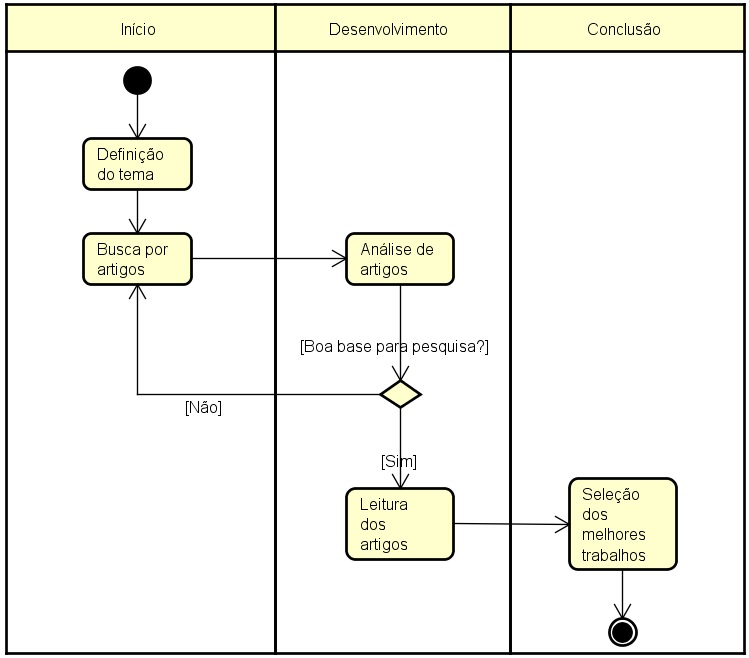
\includegraphics[width=0.9\textwidth]{imagens/diagrama.jpg}
	\caption{Diagrama de sequência indicando as etapas de seleção de artigos para a pesquisa.}
	\label{fig:diagrama}
\end{figure}

Como critérios de seleção e ordenação para a pesquisa, a revisão escolheu os artigos com maior número de citações e relevância para a área. 

O principal critério de seleção foi a proximidade com o tema destacado na introdução deste trabalho, onde a detecção de fraudes deveria ser a principal abordagem do artigo encontrado.

Realizando uma exceção, os principais artigos que tratam do tema de detecção de fraudes foram inclusos no estudo para serem utilizados, principalmente, na seção do referencial teórico, pois eram encontrados como referência na maioria dos trabalhos atuais.

Foram excluídos da revisão os artigos que fugiam do tema proposto, não possuíam citações ou relevância nas bases de dados ou eram anteriores ao ano de 2006. Os critérios de exclusão estão elencados abaixo. Foram excluídos da seleção os artigos contendo assuntos relacionados a detecção de fraudes em:

\begin{itemize}
	\item Imagens, vídeos ou impressões físicas;
	
	\item Contextos biológicos, como análises de DNA e moléculas;
	
	\item Componentes eletrônicos; 	
	
	\item Dispositivos de segurança eletrônica relacionados a vírus, \emph{firewalls} e \emph{cyber} ataques.
\end{itemize}

Para esta revisão sistemática, obteve-se foco em detecção de fraudes em dados computacionais como números e informações em tabelas, arquivos de texto, planilhas eletrônicas, etc. Isso justifica a exclusão de artigos tratando de áreas como processamento de imagens, biologia, eletrônica e segurança de redes de computadores.

Para a busca de publicações, foram considerados somente trabalhos que realizaram uma revisão no Estado da Arte em detecção de fraude, na língua inglesa e publicados no período entre 2006 e 2016. As palavras chave \emph{fraud detection survey} foram utilizadas para a busca, que obteve artigos selecionados com a leitura na respectiva ordem: título, resumo e artigo completo. Foram considerados somente trabalhos em que nenhum novo método era apresentado ou testado. Portanto, somente revisões sistemáticas na literatura da área foram inclusas.

Na primeira fase da pesquisa, foi considerada a utilização da combinação das palavras chave a seguir, que foram eliminadas da metodologia:

\begin{itemize}
	\item \emph{fraud detection AND state of art OR systematic review OR meta analysis};
	
	\
	\item \emph{anomaly detection AND survey OR state of art OR systematic review OR meta analysis};
	
	\
	\item \emph{outlier detection AND survey OR state of art OR systematic review OR meta analysis}; 	
	
	\
	\item \emph{deception detection AND survey OR state of art OR systematic review OR meta analysis}.
\end{itemize}

Os resultados contendo os temas \emph{anomaly, outlier} e \emph{deception detection} juntamente com \emph{survey} retornaram trabalhos duplicados a pesquisa com as palavras chave \emph{fraud detection survey} ou fora do escopo da pesquisa, onde a grande parte foram eliminados da seleção através dos métodos de exclusão citados anteriormente. Por esta razão, as palavras chave não foram consideradas para a pesquisa de artigos.

Outras palavras que podem significar revisões sistemáticas na língua inglesa são \emph{state of art, systematic review} ou \emph{meta analysis}. Contudo, a utilização dessas palavras chave também se mostrou obsoleta em comparação à palavra \emph{survey}, pois trouxeram muitos resultados duplicados ou em áreas indesejadas para esta revisão sistemática, como processamento de imagens, biologia, eletrônica e segurança de redes de computadores.

No início da revisão sistemática, foram encontrados 101 artigos com potencial para estruturar este trabalho. Destes, dois não estavam disponíveis para consulta. Após a leitura do título dos 99 artigos restantes, 49 foram excluídos. Posteriormente, seguindo os critérios de exclusão, foi realizada a leitura do resumo dos artigos. Destes, 22 trabalhos foram selecionados para prosseguir a revisão sistemática proposta por este trabalho. Os trabalhos estão divididos entre conferências e revistas, conforme demonstra a Tabela \ref{tab:conferenciasrevistas}.

% For tables use
\begin{table}
	% table caption is above the table
	\caption{Artigos publicados em conferências e revistas}
	\label{tab:conferenciasrevistas}       % Give a unique label
	% For LaTeX tables use
	\begin{tabular}[!Ht]{lll}
		\hline\noalign{\smallskip}
		Categoria & Quantia & Porcentagem  \\
		\noalign{\smallskip}\hline\noalign{\smallskip}
		Conferência & 12 & 55\% \\
		Revista & 10 & 45\% \\
		\noalign{\smallskip}\hline
	\end{tabular}
\end{table}

\section{Estado da Arte}
\label{sec:4}

Esta seção irá apresentar os estudos de autores na área de detecção de fraudes. Conforme descrito na seção de metodologia, foram considerados artigos que realizaram um levantamento na literatura sobre o tema.

Em uma recente publicação, \cite{Abdallah2016} elencaram as áreas mais presentes em trabalhos anteriores e as tecnologias mais utilizadas em cada contexto. Segundo os autores, fraudes ocorridas em bancos compõem 53\% dos estudos, seguido seguradoras (31\%), comércio eletrônico (10\%) e sistemas de telecomunicações (6\%). O gráfico com as informações está demonstrado na Figura \ref{fig:fraudespopulares}. 

\begin{figure}[!ht]
	\centering
	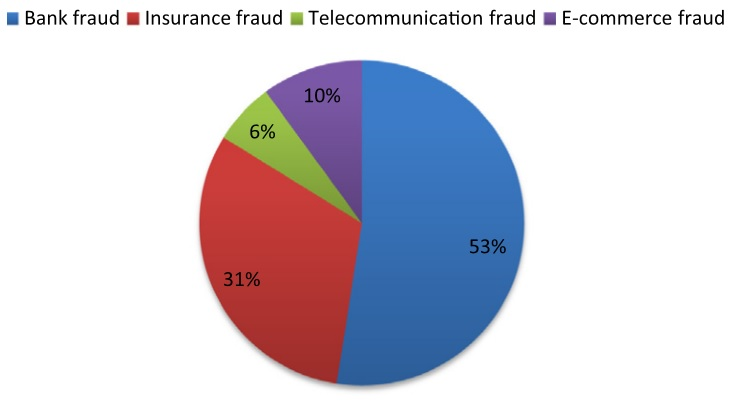
\includegraphics[width=0.9\textwidth]{imagens/fraudespopulares.jpg}
	\caption{Áreas com maior pesquisa em detecção de fraudes. Fonte: \cite{Abdallah2016}}
	\label{fig:fraudespopulares}
\end{figure}

De acordo com o \emph{Basel Committee on Bank Supervision}, existem fraudes de nível interno e externo. Fraudes em nível interno se referem às ocorridas quando empregados cometem fraudes contra a própria organização. Fraudes de nível externo correspondem a clientes ou indivíduos distantes das organizações que obtém proveito de falhas variadas \citep{Abdallah2016}.

Ainda conforme \cite{Abdallah2016}, as fraudes cometidas no contexto geral estão a crescer. De 2011 para 2016, obteve-se um acréscimo de 15\% nas fraudes cometidas em sistemas de telecomunicações.

\cite{Flegel2010} indicam que na indústria, a abordagem de detecção de fraudes não reflete à grande importância que a literatura dá para o tema. Fora do contexto acadêmico, a maior parte do processo de descobrir uma fraude é realizado por um humano, que utiliza ferramentas populares para controle de dados, como planilhas eletrônicas \emph{Microsoft Excel} ou \emph{OpenOffice Calc}. 

Os autores ressaltam que as tecnologias para detectar e coibir tentativas de invasão em sistemas de redes de computadores não podem ser comparadas - ou suas técnicas utilizadas - com detecção de fraudes em dados financeiros. \cite{Flegel2010} diferenciam as características de dados financeiros como estruturas definidas de uma forma diferente com usuários tentando atacar \emph{hardwares} de computadores.

\cite{Bansal2016} identificam as abordagens da detecção de fraudes como aplicações para detecção de fraudes em: cartões de crédito, seguradoras, sistema interno de empresas, sistema médico e de saúde e equipamentos industriais. O artigo apresenta as tecnologias para resolver os problemas apresentados, com enfoque na detecção de \emph{outliers}. 

Categorizando os \emph{outliers}, os autores denominam: \emph{Point Outliers, Contextual Outliers} e \emph{Collective Outliers}, que são os \emph{outliers} individuais, fora de padrão por contexto ou que realizam uma formação de cartel fora do padrão esperado, respectivamente. \cite{Bansal2016} ainda indicam que para detectá-los, as formas mais difundidas na literatura são: \emph{Distance based outlier detection, Clustering based outlier detection, Density based outlier detection} e \emph{Depth based outlier detection}. As características de cada técnica será apresentada posteriormente neste trabalho.

\cite{Pejic-Bach2010} e \cite{Raj2011} analisaram trabalhos que utilizaram algoritmos destinados a detectar fraudes. Com a pesquisa, constatam uma grande frequência na utilização de determinadas abordagens, como as técnicas de redes neurais, lógica \emph{fuzzy}, algoritmos genéticos, computação evolucionária, (ou evolutiva) programação genética, e otimização por nuvem de partículas. \cite{Raj2011} constataram, além das técnicas apresentadas anteriormente, os métodos de aprendizado por Inferência Bayesiana, Teoria de Evidência de Dempster-Shafer, \emph{BLAST-SSAHA Hybridization} e Modelo oculto de Markov.

\subsection{Resposta às principais perguntas}

\begin{itemize}
	\item \textbf{QP1:}\textit{"Quais são as áreas de detecção de fraudes mais estudadas na literatura?"};
	
	\textbf{RQP1:}
	
	\
	\item \textbf{QP2:}\textit{"Como a literatura categoriza as técnicas de detecção de fraudes?"};
	
	\textbf{RQP2:}
	
	\
	\item \textbf{QP3:}\textit{"Quais problemas aparecem com mais frequência segundo os autores?"};
	
	\textbf{RQP3:}
	
	\
	\item \textbf{QP4:}\textit{"Como os autores fizeram para testar e validar suas pesquisas?"};
	
	\textbf{RQP4:}
	
	\
	\item \textbf{QP5:}\textit{"Em que área há pouca abordagem no estudo de detecção de fraudes?"};
	
	\textbf{RQP5:}
	
	\
	\item \textbf{QP6:}\textit{"Há novas abordagens e espaços para futuras pesquisas na área?"}.
	
	\textbf{RQP6:}
	
\end{itemize}

\section{Discussão}
\label{sec:5}

Nas seções anteriores, foi possível observar o estado das pesquisas relacionadas à detecção de fraudes. Conforme as observações realizadas, esta seção visa discutir os fatores em comum entre os trabalhos.

% For tables use
\begin{table}
	% table caption is above the table
	\caption{Áreas mais abordadas pelos autores e as técnicas mais utilizadas.}
	\label{tab:XX}       % Give a unique label
	% For LaTeX tables use
	\begin{tabular}[!Ht]{lll}
		\hline\noalign{\smallskip}
		Autores & Áreas & Técnicas  \\
		\noalign{\smallskip}\hline\noalign{\smallskip}
		XX & XX & XX\% \\
		XX & XX & XX\% \\
		\noalign{\smallskip}\hline
	\end{tabular}
\end{table}

O principal desafio apontado pela maioria dos autores diz respeito à evolução das técnicas utilizadas pelos fraudadores para burlar os sistemas. Em estudos constatados por corporações bancárias, o comportamento esperado por fraudadores demonstrou uma mutação quando os criminosos entenderam as técnicas para detectá-los \citep{Bolton2002}. Indivíduos que em outrora utilizavam cartões de crédito somente para efetuar compras com a intenção de não pagá-las, perceberam que poderiam pagar as compras iniciais para serem classificados como usuários comuns, e assim possuir maior margem para fraudar no futuro.

Entendendo o problema da mutação nas técnicas criminosas, constata-se que a engenharia de software tradicional possui um processo de produção padrão, onde ocorre etapas de análise, projeto, codificação, implementação e testes \citep{sommervillesoftware}. Dessa maneira, a constante evolução das características de usuários fraudulentos pode se tornar um desafio para englobar um modelo de desenvolvimento tradicional de software. 

Ao analisar os trabalhos desenvolvidos na área de detecção de fraudes, não foi possível constatar a presença de um conjunto de dados padrão que pudesse ser utilizado por diversos algoritmos para computação e comparação de valores. Em seus trabalhos, os autores utilizaram dos mais variados tipos de dados, sendo possível identificar duas grandes características em comum: houveram autores que utilizaram dados controlados, possivelmente criado por eles; e dados reais, onde utilizaram suas técnicas e algoritmos em informações providas de empresas e problemas reais. 

O empecilho, porém, está no fato em que os autores comparam os seus algoritmos com os já existentes na literatura utilizando os dados que lhes são convenientes. Esta revisão sistemática propõe como sugestão para trabalhos futuros desenvolver e apresentar um conjunto de dados que possa servir como um \emph{benchmark}, onde diversos pesquisadores realizem seus estudos nos mesmos ambientes, para fim de padronização dos testes. 

\section{Conclusão}
\label{sec:6}

Este trabalho realizou a revisão sistemática na área de detecção de fraudes. Pesquisas realizadas para dar o panorama na área foram estudadas e discutidas. Em conclusão, o trabalho indica que a área, embora muito estudada, ainda concentra amplo poder para novas pesquisas. Obtendo os principais artigos publicados na área, constatou-se um grande crescimento de publicações na área acadêmica após o ano de 2010. Isto demonstra que o assunto está em crescimento de interesse.

Em trabalhos futuros, almeja-se continuar a pesquisa em detecção de fraudes, aplicando técnicas para auxiliar a auditoria e controle de órgãos públicos a descobrir irregularidades em dados.

Após a finalização da revisão sistemática, espera-se a publicação dos resultados obtidos na revista Data Mining and Knowledge Discovery, a qual possui a classificação de qualidade Qualis B1, elencada pela CAPES em sua última análise. 

	% BibTeX users please use one of
	\bibliographystyle{spbasic}
	\bibliography{minhabibliografia2}
	
	\begin{appendices}
			Conforme visto na Figura \ref{fig:cronograma}, o escopo do trabalho foi delimitado pelas tarefas: Definir tema; Definir objetivos, justificativa e motivação; Escolher o local para publicação; Elaborar o método de pesquisa; Revisar a literatura e selecionar trabalhos; Produzir artigo científico; e Publicar o artigo finalizado. 
			
			As tarefas foram divididas entre os meses de junho a setembro e receberam a classificação: Concluída ("OK", em verde); Em andamento ("Andam.", em amarelo); e Não iniciada ("Não Inic.", em vermelho). 
			
			\begin{figure}[!ht]
				\centering
				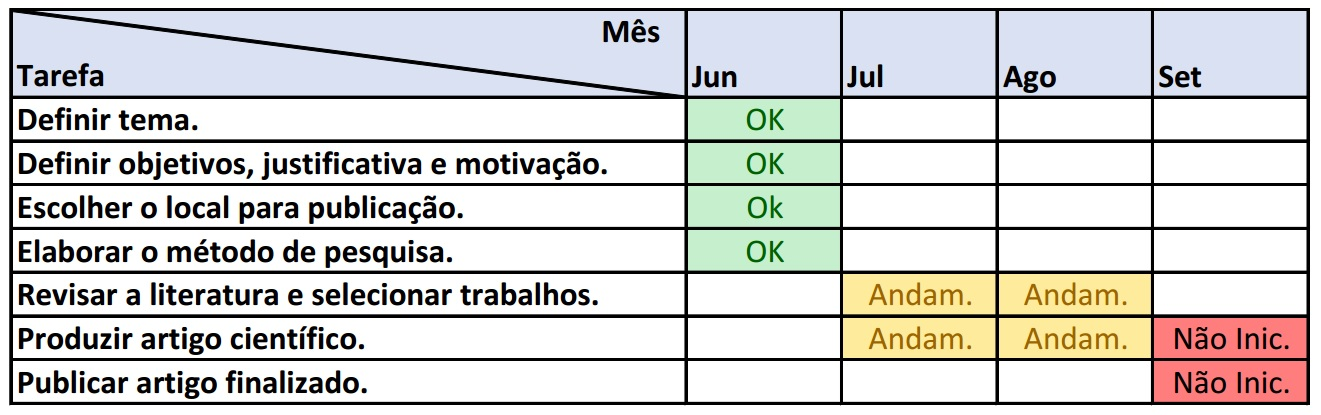
\includegraphics[width=1\textwidth]{imagens/cronograma2.jpg}
				\caption{Cronograma do planejamento do projeto.}
				\label{fig:cronograma}
			\end{figure}
	\end{appendices}
	
\end{document}